\documentclass{article}
\usepackage[T1]{fontenc}
\usepackage{neurips_2025}
\usepackage{graphicx}
\usepackage{booktabs}
\usepackage{amsmath,amssymb}
\usepackage{microtype}
\usepackage{hyperref}
\hypersetup{hidelinks}

\title{A Reproducible Benchmark for Earned vs Enforced Measurement Consistency in Dynamic Interferometric Imaging}

\author{%
  Anonymous Author(s)\\
  Anonymous Institution
}

\begin{document}

\maketitle

\begin{abstract}
Structured inverse problems are often evaluated on coefficients that were either directly observed or explicitly restored by a data-consistency layer, which makes it difficult to tell whether a model truly learned to recover unmeasured information. We propose a reproducible benchmark for \emph{earned} versus \emph{enforced} measurement consistency under structured Fourier missingness. Dynamic VLBI is the motivating case because it is extreme: sparse complex-valued measurements, non-Cartesian Fourier coverage, and time variability \citep{EHT2019M87I,ngEHTScience}. The benchmark fixes deterministic support-target manifests, three holdout families, release-aware public validation, and paired-bootstrap reporting. On the released synthetic breadth matrix, the earned-consistency reference model EMC is strongest in all 12 family-support cells, while public EHT validation reveals release-dependent transfer limitations that become partly but not uniformly smaller under test-time optimization. Those mixed public outcomes are useful because they expose the residual synthetic-to-real gap rather than hiding it behind pooled averages. The protocol is not specific to VLBI; it applies directly to time-varying MRI settings in which extrapolation to unobserved Fourier coefficients is equally central.
\end{abstract}

\section{The benchmark question}

The central question is simple: can a reconstruction method recover structured Fourier coefficients that were \emph{never shown} to the model and \emph{never restored} by a support-set data-consistency operator? We call success on that task \emph{earned} measurement consistency. By contrast, \emph{enforced} consistency arises when observed coefficients are reinserted explicitly, so low error on those same coefficients is no longer evidence of learned extrapolation. This distinction matters across structured inverse problems, but dynamic VLBI makes it unusually sharp because sparse time-varying baselines leave little room to hide evaluation leakage \citep{EHT2019M87IV,EHT2022SgrAIII}.

\section{Protocol}

Our protocol fixes deterministic support-target manifests under three structured missingness families: baseline-track blocks, scan-segment blocks, and station dropout. Each family is evaluated at support fractions of 20, 40, 60, and 80 per cent on a common $64\times64$ grid. The benchmark release stores split manifests, configuration manifests, results manifests, seeds, paired-bootstrap summaries, public-EHT release metadata, and figure/table generation scripts. Released public validation spans four official calibrated-data products: M87 2017, M87 2018, 3C279 2017, and Centaurus A 2017.

\section{Key results}

Table~\ref{tab:synthetic} summarizes the synthetic benchmark signal. EMC is the strongest learned method in all 12 cells of the released breadth matrix, and on the baseline-track 20 per cent slice it reduces held-out visibility-error power by 63.3 per cent relative to residual refinement, the strongest enforced learned comparator in that slice. A bounded five-seed follow-up narrows the method claim, but it does not weaken the benchmark claim: the protocol is informative precisely because it separates favorable released breadth from stricter robustness.

\begin{table}[t]
\caption{Synthetic benchmark summary.}
\label{tab:synthetic}
\centering
\small
\begin{tabular}{p{0.41\linewidth}p{0.47\linewidth}}
\toprule
Result & Value \\
\midrule
Released breadth matrix & EMC best learned model in 12/12 family-support cells \\
Baseline-track 20\% support & 63.3\% lower held-out visibility-error power than residual refinement \\
Five-seed baseline-track study & Residual refinement strongest mean learned comparator in 4/4 support fractions \\
Conformal UQ on EMC & Mean empirical 90\% coverage $=85.8\%$; mean interval width $=0.168$ \\
\bottomrule
\end{tabular}
\end{table}

Table~\ref{tab:public} shows the public-EHT reality check. Test-time optimization (TTO) helps on M87 2017 and strongly on 3C279 2017, but degrades M87 2018 and Centaurus A 2017. The public story is therefore benchmark-strengthening rather than method-conclusive: structured hold-out evaluation continues to separate regimes after leaving the synthetic domain. The add-on cycle also introduces a bounded Diffusion Posterior Sampling (DPS) comparator \citep{Chung2023DPS}, which gives an earned-consistency diffusion baseline without access to held-out target measurements.

\begin{table}[t]
\caption{Public EHT baseline-track release summary with TTO. Positive uplift means lower held-out visibility RMSE than plain EMC.}
\label{tab:public}
\centering
\small
\begin{tabular}{lcc}
\toprule
Release & EMC-TTO uplift & Release-level outcome \\
\midrule
M87 2017 & +0.0696 & Improved, but Tikhonov remains strongest mean model \\
M87 2018 & -0.0833 & Degraded under adaptation \\
3C279 2017 & +0.2275 & Best release-level transfer case; EMC-TTO wins \\
Centaurus A 2017 & -0.1862 & Degraded under adaptation \\
\bottomrule
\end{tabular}
\end{table}

\begin{figure}[t]
\centering
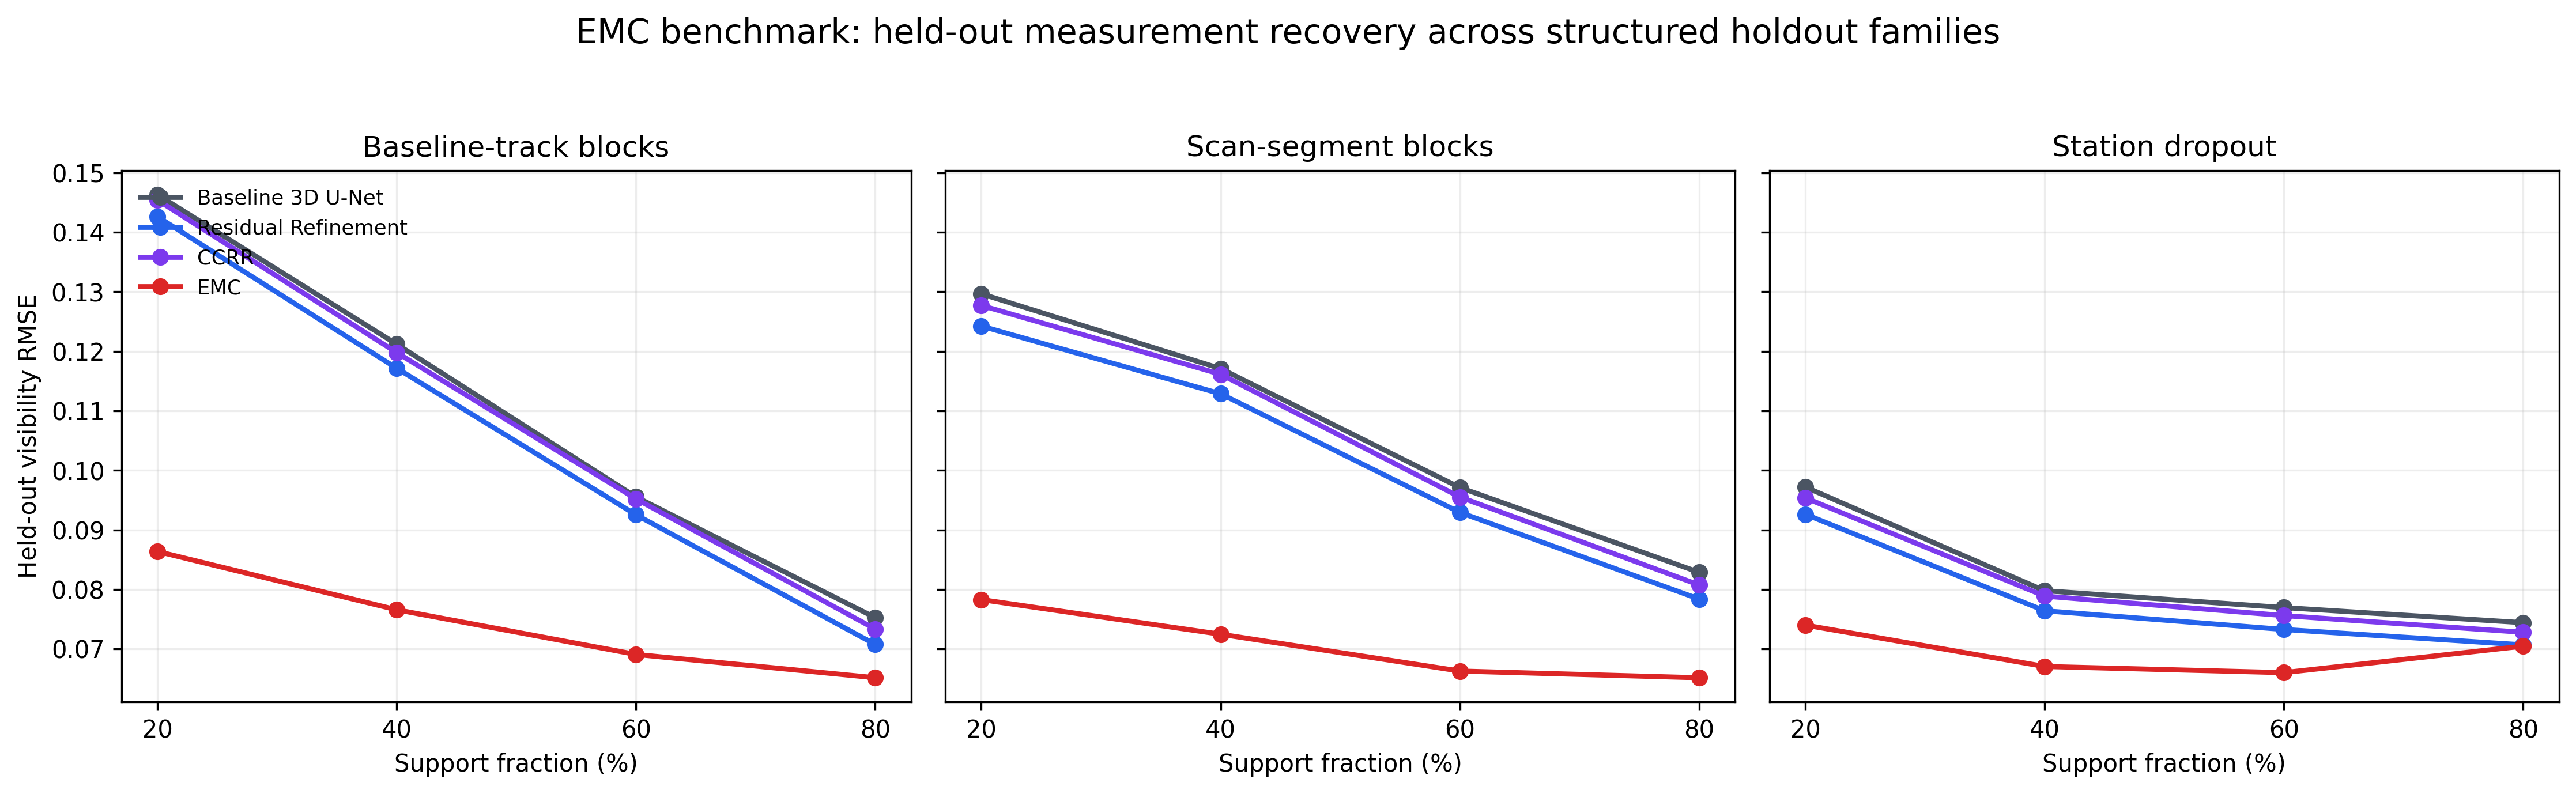
\includegraphics[width=\linewidth]{../figures/fig02_emc_benchmark_support_curve.png}
\caption{Support-fraction curves for the released synthetic benchmark. The main signal is not that one architecture always wins, but that earned-vs-enforced evaluation yields a stable and reproducible separation across structured missingness families.}
\label{fig:support-curves}
\end{figure}

\section{Cross-domain applicability}

The protocol is not unique to VLBI. Cardiac cine MRI has the same mathematical structure: a time-varying source observed through undersampled Fourier measurements with structured missingness across time. Methods that enforce k-space agreement at observed frequencies need not generalize to unobserved frequencies across cardiac phases. FastMRI-style cine benchmarks could therefore test the same earned-versus-enforced protocol in a domain with image-domain ground truth and higher clinical stakes \citep{Zbontar2018fastMRI,Cui2024SPIRITDiffusion}. The same logic also connects naturally to recent diffusion-based interferometric imaging work in astronomy \citep{Lai2025ConditionalDiffusionVLBI}. In that sense, VLBI is the extreme structured-inverse-problem case, not the only one.

\section{Conclusion}

The benchmark release makes one point reproducibly: agreement on observed coefficients is not enough. In dynamic interferometric imaging, the scientifically relevant question is whether a method can recover unobserved coefficients under structured missingness, and whether that ability survives contact with released public measurements. The same benchmark logic extends naturally to other time-varying Fourier inverse problems, including cardiac cine MRI. We release the manifests, artifact builders, theory note, and public-EHT validation suite to support that broader comparison agenda.

\bibliographystyle{plainnat}
\bibliography{references}

\end{document}
